\chapter{Introduction}

\section{Some Words About this Document}
\subsection{Embedded Listings}

Some of the listings later on in this manual are meant to be copied and pasted into external editors. It is okay to do this for short code snippets but it is often to tedious with longer scripts. Therefore we decided to embed the corresponding scripts into the PDF, like attachments to an email. Unfortunately not all PDF viewers are capable of retrieving the attached listings. Some viewers which support this feature (cf Fig. \ref{fig:pdf_attach}) include Adobe Reader since version 6.0, Foxit Reader, Okular etc.

\begin{figure}[htb] 
  \centering 
  \subfloat[Acrobat Reader.]{
    \label{fig:pdf_attach_acroread}
    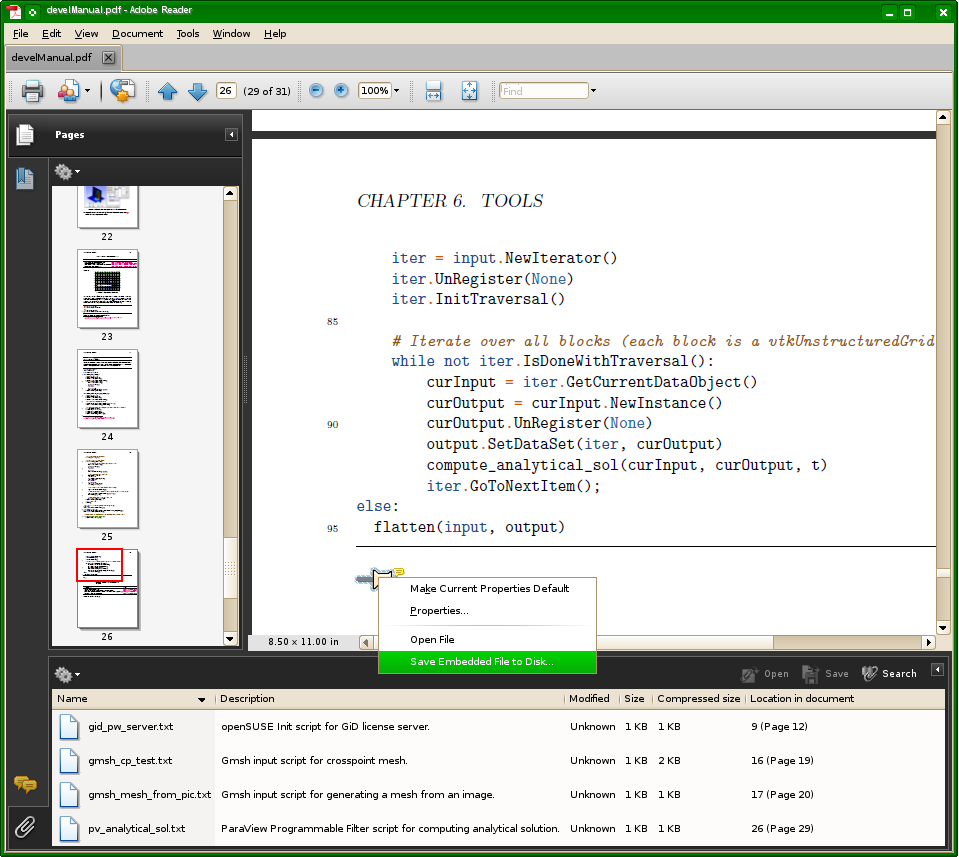
\includegraphics[width=7cm]{pics/pdf_attach_acroread}
  }
  \qquad
  \subfloat[Okular.]{
    \label{fig:pdf_attach_okular}
    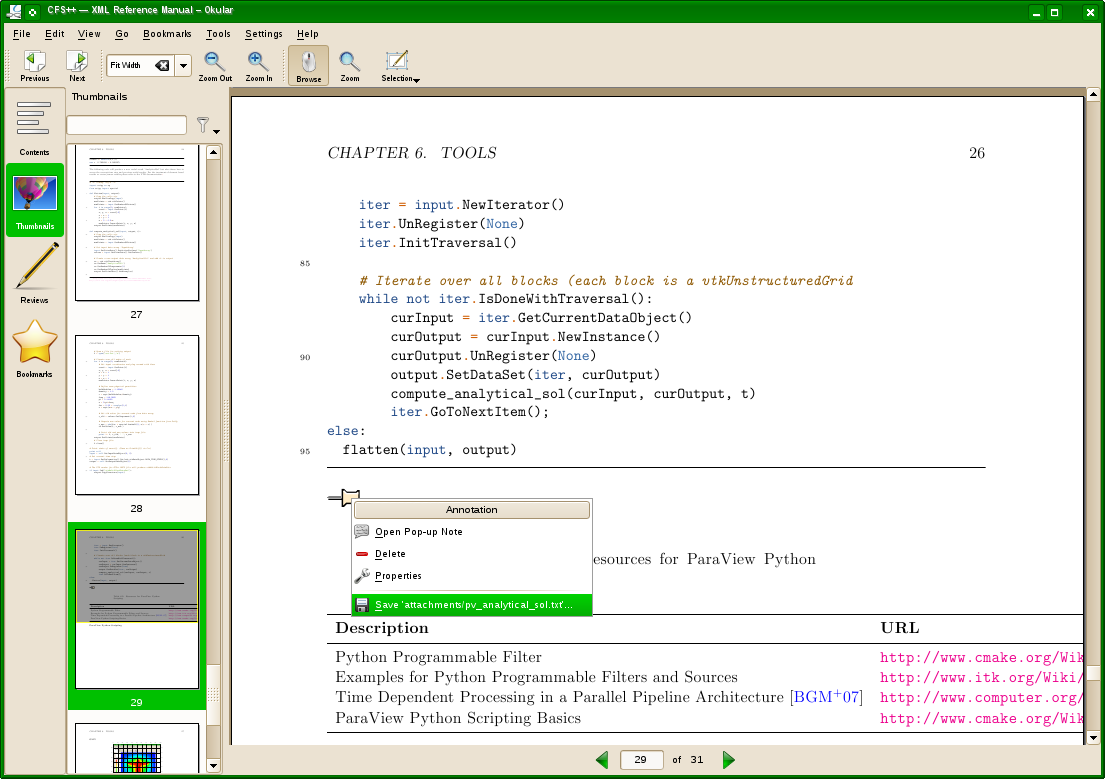
\includegraphics[width=7cm]{pics/pdf_attach_okular} 
  }
  \qquad
  \subfloat[Foxit Reader.]{
    \label{fig:pdf_attach_foxit}
    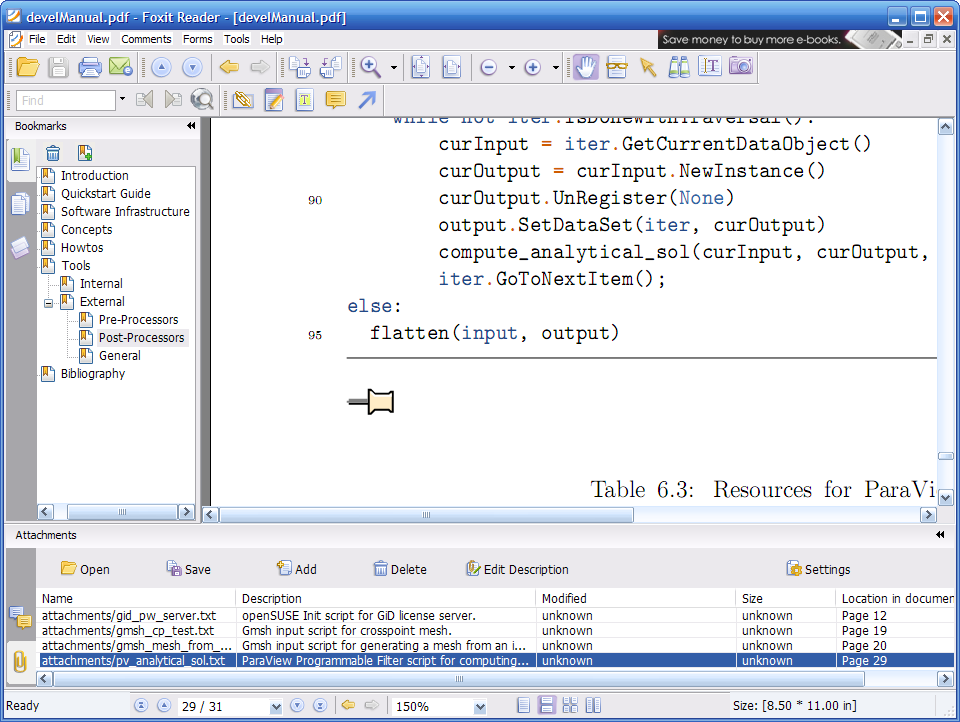
\includegraphics[width=7cm]{pics/pdf_attach_foxit}
  }
  \caption{Extracting PDF attachments using different viewers.}
  \label{fig:pdf_attach}
\end{figure}
